\setcounter{page}{1}
\chapter{INTRODU\c{C}\~AO}  %%Nesta linha, dentro de { }, digita-se em CAIXA ALTA, como apresentado aqui
\label{chap:01}

O \textit{software} está inserido em praticamente todos os aspectos de nossas vidas, podendo colaborar para a otimização da linha de produção de industrias, melhorar a gestão de empresas ou até mesmo mudar a forma como as pessoas se relacionam. Diante desta grande demanda, o \textit{software} e todos os artifícios envolvidos em seu desenvolvimento precisam ser constantemente aperfeiçoados, desta forma, a engennharia de \textit{software} surgiu com o objetivo de aplicar princípios de engenharia na especificação, no desenvolimento e na manutenção de \textit{software}.

A grande demanda para construções de \textit{softwares} cada vez mais complexos e com mais funcionalidade, acarretou em projetos extensos, com bases de códigos enormes, que desencadeiam diverssos problemas para o gerenciamento, por exemplo, erros de estimativa, custos elevados e até mesmo desgastes emocionais e desmotivação dos engenheiros envolvidos. Para minimizar os problemas de projetos extensos, a engennharia de \textit{software} possui o conceito de modularidade, nele é enfatizado que o \textit{software} modular pode ser melhor gerenciado que o monolítico. Além disso, a modularização possibilita que o \textit{software} seja planejado mais facilmente e que os custos para mautenção sejam reduzidos.

Diferente da abordagem monolítica o desenvolvimento de \textit{software} baseado em \textit{microservices} visa construir vários \textit{softwares} menores, com propósitos específicos, que se comunicam trocando informações para resolver problemas complexos. Básicamente neste modelo a modularização é intencificada visando simplificar ao máximo a complexidade dos projetos. Entretanto muitas vezes o projeto não se iniciou seguindo o modelo de \textit{microservices}, desta forma, muitas vezes os \textit{microservices} são extraidos de um \textit{software} maior, em muitos casos de um monolito.

Este trabalho visa propor um modelo para extração de \textit{microservice} de um \textit{software} monoítico, baseado em um cenário real de uma empresa de tecnologia, que está em amplo crescimento, e que por possuir um \textit{software} monolítico, enfrenta vários problemas ocasionados pelo modelo de arquitetura de \textit{software} adotado.

\section{Objetivo}

O objetivo deste trabalho é propor um modelo de arquitetura de \textit{software} que possibilite a extração gradativa de \textit{microservices} de um \textit{software} monoítico, sem que haja a necessidade de reescrever toda a aplicação no novo modelo, ou seja, deverá ser possível além de evoluir a arquitetura de \textit{software} dando suporte a evolução constante do produdo, desta forma, possibilitando que novas funcionalidades sejam adicionadas e mantidas.

\section{Justificativa}

Na ContaAzul, empresa localizada em Joinville, todo o \textit{software} (ContaAzul) está centralizado em um único projeto e cada um dos vários times de desenvolvimento que a empresa possui é responsável por um conjunto de funcionalidades deste \textit{software}, desta forma todos os times trabalham dando manutenção e inserindo novas funcionalidades na mesma aplicação monolítica.

Tendo mais de 50 engenheiros de  o \textit{software}, diariamente executando do processo de desenvolvimento na mesma grande base de código do ContaAzul, fica evidenciado os problemas da aplicação monolítica, refletidos em atrasos para finalizações de tarefas do processo de desenvolvimento. A Figura \ref{fig:01} apresenta o processo de desenvolvimento atual adotado pelos times da ContaAzul.

\begin{figure}[hb]
	\begin{center}
		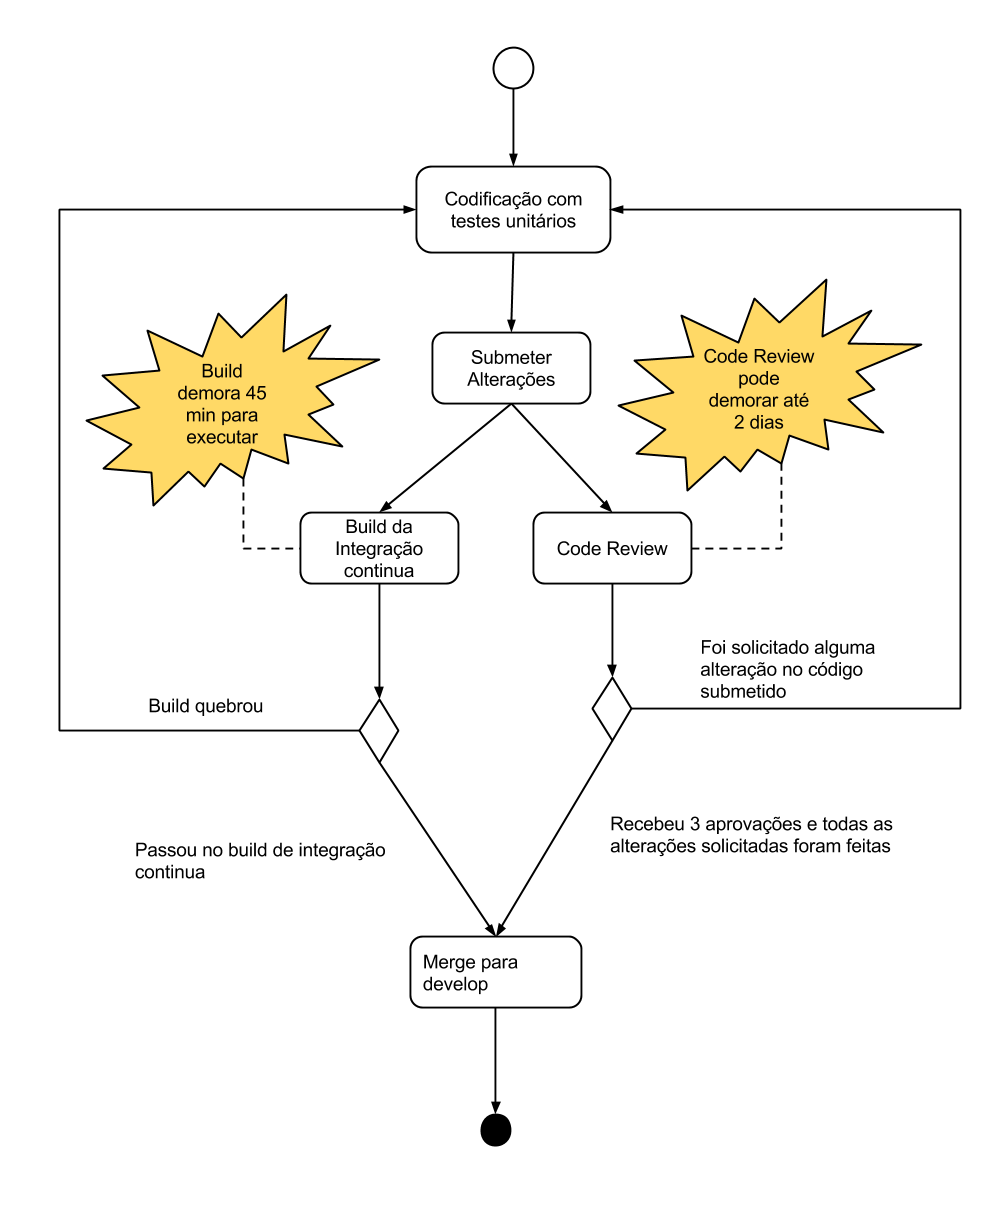
\includegraphics[width=12cm]{assets/processo_desenvolvimento.png}
		\caption{Processo de Desenvolvimento dos Times da ContaAzul}
		\label{fig:01}
	\end{center}
\end{figure}

Na Figura \ref{fig:01} são evidenciado os 2 problemas mais custosos do processo, foi decidido pelo time de engenharia da empresa que o custo para alteração do processo e readequação de todo o model de trabalho, não resolveria o causa rais dos problemas, o \textit{software} monolítico.

Desta forma, pensando a logo prazo, foi identificado que a migração para um modelo de \textit{microservices} poderia ser uma proposta melhor para solucionar os problemas apontados.

\section{Estrutura do Trabalho}

// TODO: Definir a estrutura do trabalho 